\documentclass[12pt,a4paper]{report}

\usepackage[utf8]{inputenc}
\usepackage[T1]{fontenc}
\usepackage[spanish]{babel}
\usepackage[left=3cm,right=2.5cm,top=3cm,bottom=2cm]{geometry}
\usepackage{graphicx}
\usepackage{enumitem}
\usepackage{caption}
\usepackage{pdfpages}

\graphicspath{{imagenes/}}
\pagestyle{plain}
\setlength{\parindent}{1.5em}
\setlength{\parskip}{0pt}
\captionsetup[figure]{font=normalsize,labelfont=normalfont,labelsep=colon}

% Fragmento del expediente: conserva la numeración del PDF de referencia.

\begin{document}

\newgeometry{left=2cm,right=2cm,top=1.5cm,bottom=1.5cm}
\begin{titlepage}
  \centering
  \thispagestyle{empty}

  {\fontsize{25}{30}\selectfont\bfseries
    Universidad Nacional de San\\
    Antonio Abad del Cusco\par}

  \vspace{0.6cm}
  \hrule
  \vspace{0.25cm}
  {\fontsize{20}{25}\selectfont
    Facultad de Ingeniería Eléctrica, Electrónica,\\
    Informática y Mecánica\par}
  \vspace{0.25cm}
  \hrule

  \vspace{0.6cm}
  {\fontsize{17}{21}\selectfont
    Escuela Profesional de Ingeniería Informática y de Sistemas\par}

  \vspace{0.5cm}
  
\includegraphics[height=5.5cm]{logo-unsaac.png}%
  \hspace{0.4cm}%
  
\includegraphics[height=5.5cm]{logo-informatica.png}\par

  \vspace{0.8cm}
  {\fontsize{25}{30}\selectfont\bfseries
    EXPEDIENTE TÉCNICO DE\\
    OBRA\\
    Sistema de Cableado Estructurado\par}

  \vspace{0.35cm}
  {\Large\bfseries Tema: Cableado y estructurado\par}

  \vspace{0.8cm}
  {\Large Primer entregable del curso de:\par}
  {\fontsize{20}{25}\selectfont\bfseries Redes de computadoras I\par}

  \vspace{0.4cm}
  {\Large\bfseries Docente:\par}
  {\large Rony Villafuerte Serna\par}

  \vspace{0.4cm}
  {\Large\bfseries Integrantes:\par}
  \vspace{0.15cm}
  \begin{tabular}{@{}lr@{}}
    - José Francisco Quentasi Juachin & 215948\\
    - Luis Alejandro Ramos Aguirre & 225425\\
    - Hernan Washington Ramos Alata & 221989\\
    - Efrian Vitorino Marin & 160337
  \end{tabular}\par

  \vfill
  {\large 10 de agosto de 2026\par}
\end{titlepage}
\restoregeometry

\setcounter{page}{13}
\setcounter{chapter}{1}
\setcounter{section}{5}
\setcounter{figure}{3}

\section{Normas y estándares aplicados}

El diseño, suministro, instalación y certificación de todo el sistema de
telecomunicaciones se regirá estrictamente por las normas y estándares
internacionales de la industria de cableado estructurado, así como por las
especificaciones técnicas detalladas en el presente expediente.

\begin{enumerate}[label=\arabic*.,leftmargin=2.5em,itemsep=0pt,parsep=0pt]
  \item \textbf{Estándares de Cableado Estructurado:}
    \begin{itemize}[label={},leftmargin=2.5em,itemsep=0pt,parsep=0pt,topsep=0pt]
      \item El proyecto debe cumplir con los estándares \textbf{ANSI/TIA/EIA}
        aplicables para cableado de telecomunicaciones.
      \item El cableado estructurado será instalado y certificado según la
        \textbf{Categoría 6A} para el canal completo.
      \item Las etiquetas de cables, patch cords y paneles deben seguir el
        estándar \textbf{ANSI/TIA/EIA 606B}.
      \item El sistema de cableado debe ser diseñado bajo la premisa de los
        \textbf{seis componentes clave} de la infraestructura de
        telecomunicaciones: Instalaciones de entrada, Sala de equipos,
        Canalizaciones de montantes (Back-bone), Salas de telecomunicaciones,
        Canalizaciones horizontales y Áreas de trabajo.
    \end{itemize}

  \item \textbf{Estándares de Fibra Óptica:}
    \begin{itemize}[label={},leftmargin=2.5em,itemsep=0pt,parsep=0pt,topsep=0pt]
      \item Las especificaciones y parámetros de transmisión para el cableado
        de fibra óptica están basados en las normas \textbf{TIA-568 y TIA-569}.
      \item Se recomienda el uso de fibra óptica multimodo de \textbf{50~µm}
        para cableado vertical debido a su eficiencia en distancias largas.
    \end{itemize}

  \item \textbf{Normas de Calidad y Unidades:}
    \begin{itemize}[label={},leftmargin=2.5em,itemsep=0pt,parsep=0pt,topsep=0pt]
      \item En todos los documentos del presente suministro se utilizará el
        \textbf{Sistema Métrico Internacional de Medidas}.
      \item Los materiales utilizados en la instalación, incluidos los equipos,
        deben ser \textbf{nuevos, de la mejor calidad} dentro de su clase y
        libres de defectos.
      \item El equipo en general debe funcionar sin vibraciones indebidas y con
        el mínimo ruido permitido por las normas.
      \item El revestimiento de los cables (UTP, Patch Cord y Line Cord) debe
        ser \textbf{LSZH (Low Smoke Zero Halogen)}.
    \end{itemize}

  \item \textbf{Certificación y Pruebas:}
    \begin{itemize}[label={},leftmargin=2.5em,itemsep=0pt,parsep=0pt,topsep=0pt]
      \item Se someterá a los materiales y equipos a todas las \textbf{pruebas,
        controles, inspecciones o verificaciones} prescritas para comprobar
        su cumplimiento.
      \item La certificación del cableado estructurado se realizará
        \textbf{in situ por un Certificador independiente}.
      \item Se utilizarán \textbf{probadores de campo calibrados} para la
        certificación de puntos de red y se deberá generar el reporte con los
        parámetros técnicos.
    \end{itemize}
\end{enumerate}

% Exportación vectorial del archivo PlanosIIS.dwg: vista general y láminas
% de plantas, cubiertas, cortes y elevaciones en su propio formato de papel.
% Se omiten las tramas HATCH: su conversión generaba rellenos que ocultaban
% el dibujo. La presentación está ajustada al papel, no a escala de impresión.
\clearpage
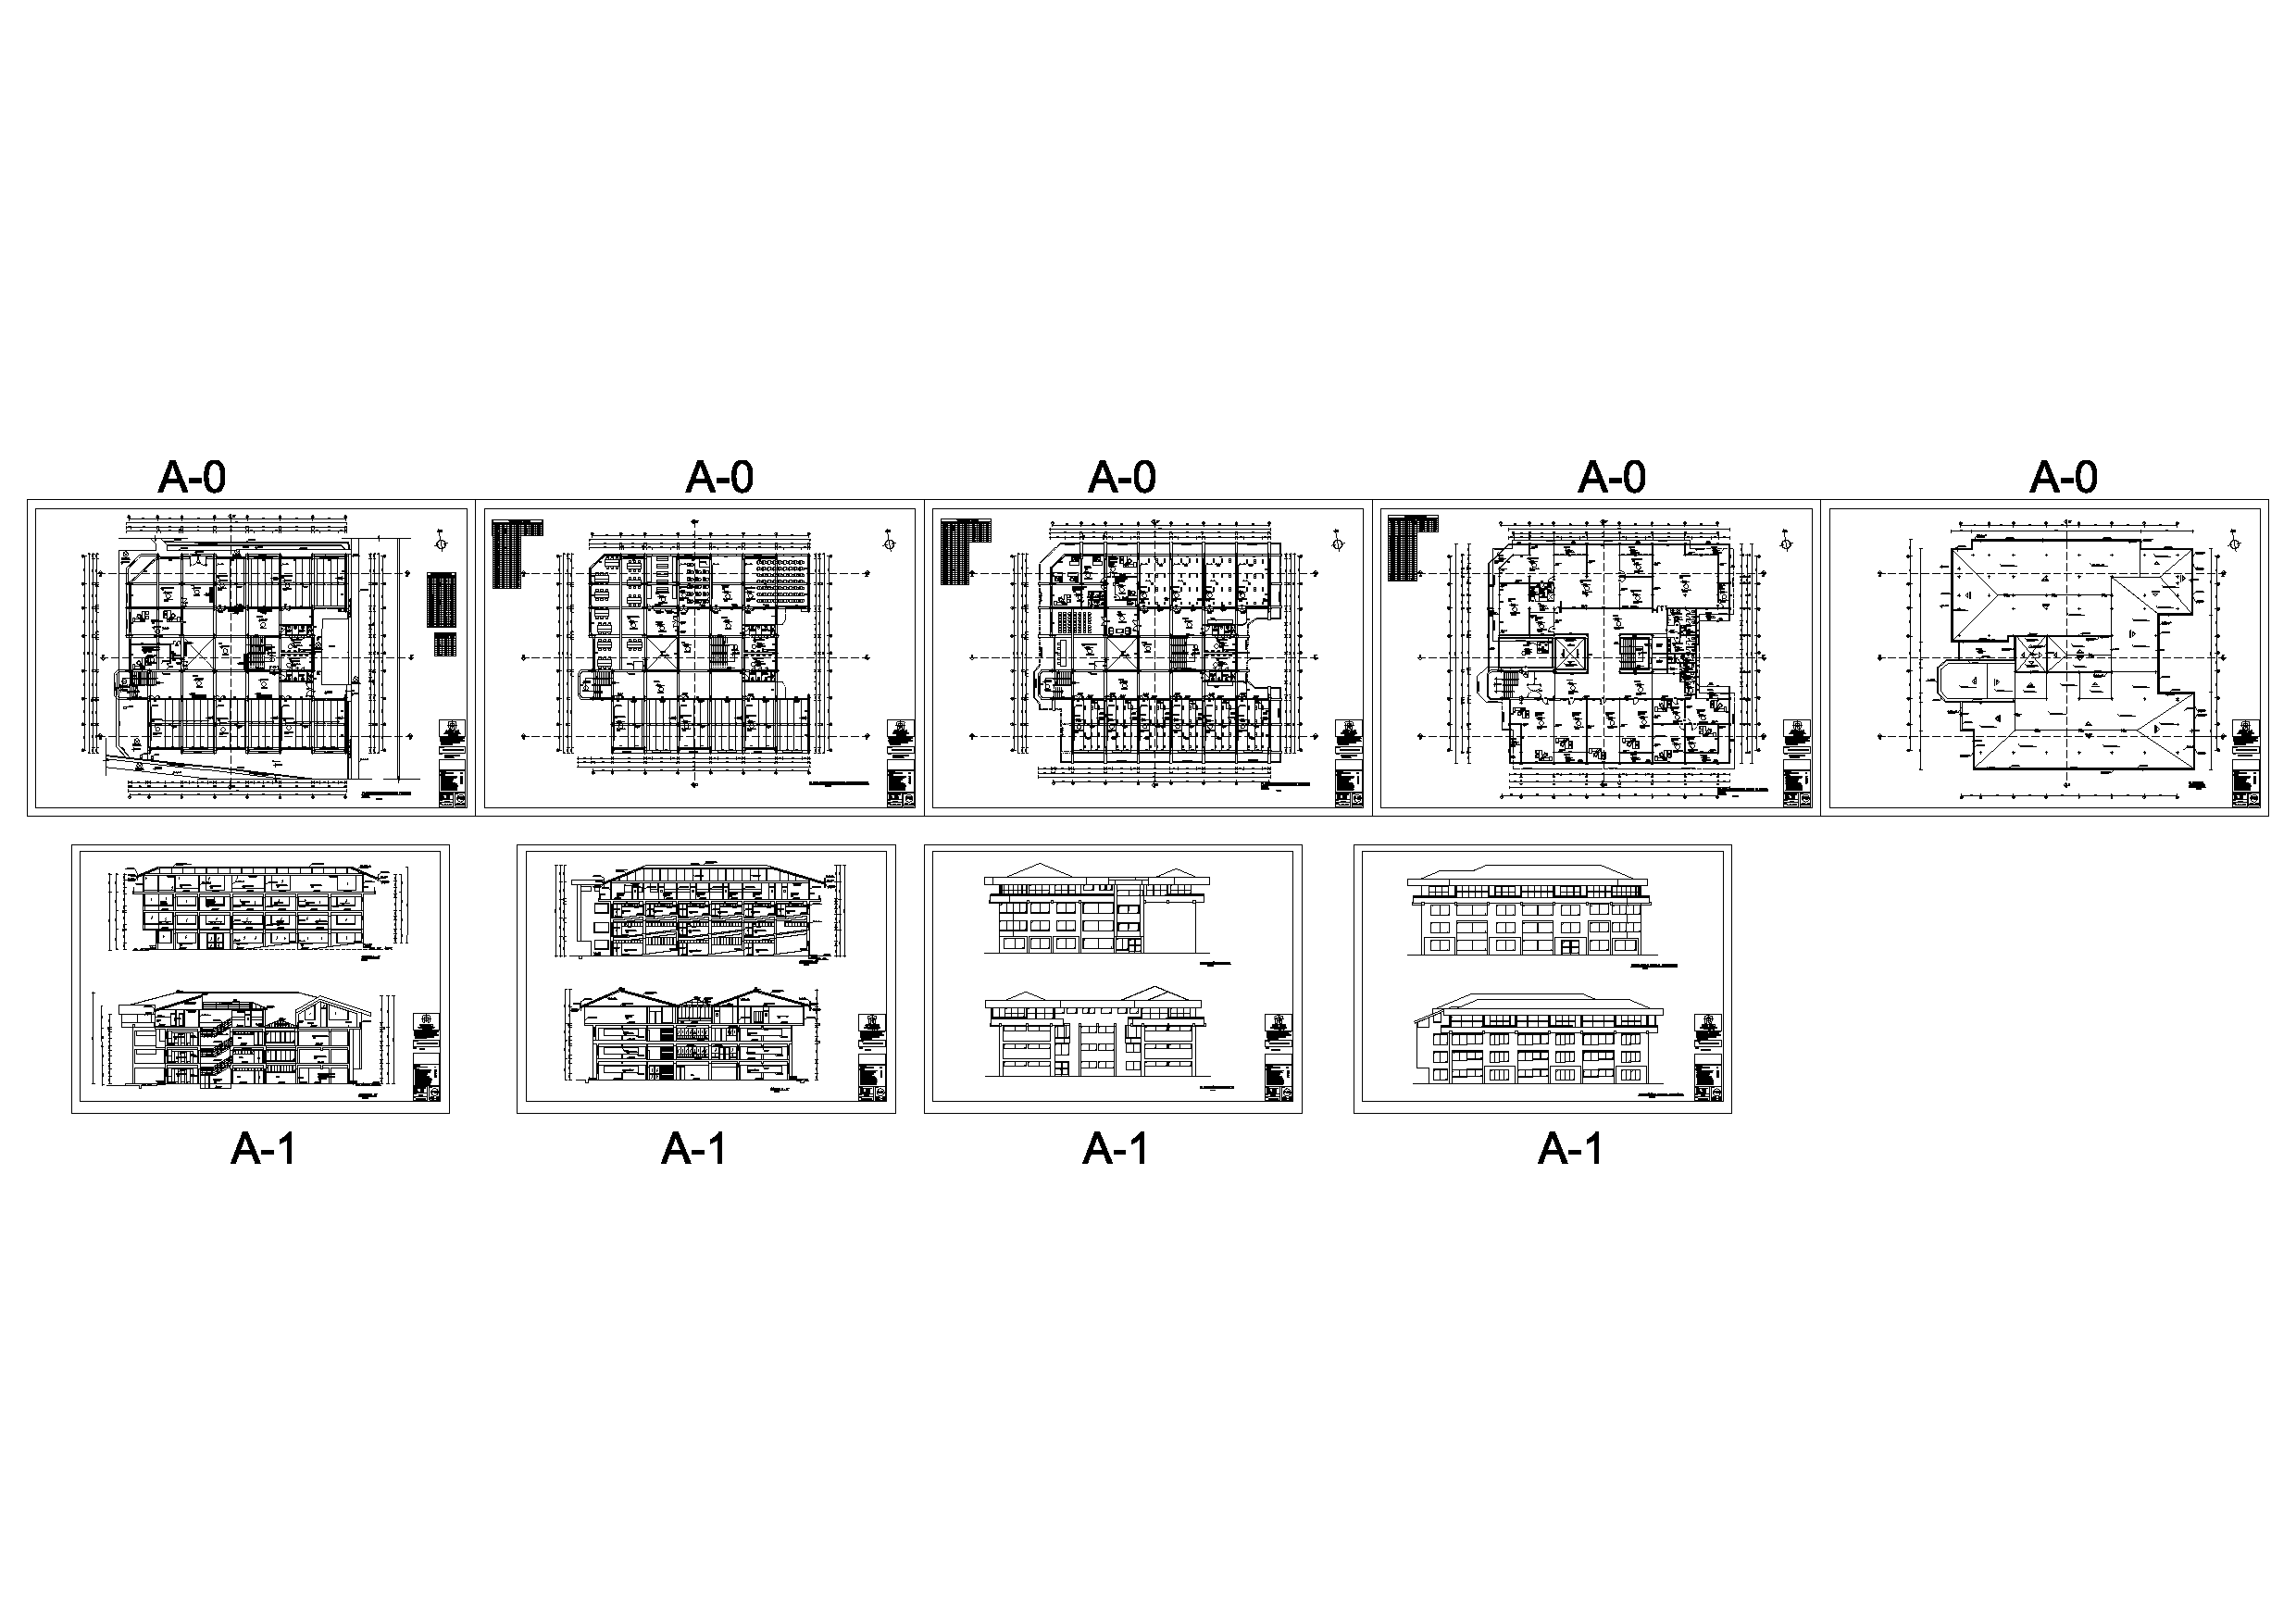
\includepdf[pages=-,fitpaper=true,pagecommand={}]{imagenes/PlanosIIS.pdf}

\end{document}
